\documentclass[12pt]{article}
\title{China -- The Empire That Did Not Bark \footnote{following the Sherlock Holmes story ``Silver Blaze'' by Sir Arthur Conan Doyle, Holmes was able to deduce that the killer of Colonel Ross's racehorse was the owner of the stable dog, the dog that did not bark. What does not happen is often as important as what does.}\\
presented at\\
Social Science History Association\\
Annual Conference\\
Vancouver, B.C.\\
November 1 - 4, 2012}

\author{Stephen C. Bannister\\
	Department of Economics\\
	University of Utah\\
	Salt Lake City, Utah 84112\\
	USA\\
	\href{mailto:steve.bannister@econ.utah.edu}{steve.bannister@econ.utah.edu}\\
	}
%\date{\today}
\date{}
\usepackage[latin1]{inputenc}
\usepackage{amsmath}
\usepackage{mathtools}
\usepackage{amsfonts}
\usepackage{txfonts}
\usepackage{amssymb}
%\usepackage{amsthm}
\usepackage{pgfpages}
\usepackage{booktabs}
\usepackage{verbatim}
\usepackage[justification=centering]{caption}
\usepackage{hyperref}

\usepackage{natbib}
%\usepackage{glossaries}
%\linespread{1.9}	% remove for single, 1.3 for 1.5 and 1.6 for 2.0. use this setting for print editing

\newtheorem{mydef}{Definition}[section]
\numberwithin{equation}{section}

\begin{document}

%\graphicspath{{./images/}}

%\bibliographystyle{plain}
	\maketitle
	
	
%\includegraphics[width=0.70\textwidth]{\url{run:http://home.utah.edu/~u0582526/images/gbpmtoelog.png}}	
\href{http://home.utah.edu/~u0582526/images/gbpmtoelog.png}{\includegraphics[width=0.70\textwidth]{http://home.utah.edu/~u0582526/images/gbpmtoelog.png}}

\end{document}

\subsection{sequence for bibliography}

pdflatex
bibtex on .bib
pdflatex
pdflatex
bibtex on .tex
pdflatex
pdflatex

\section{Notes}
11/11/12\\
soften institutional part in intro\\
add in history stuff from SHOE threads\\
in fundamental neoclassical model, note that can also be interpreted  production prices and effective demand, so surplus and distribution\\
ssha inputs